\documentclass[10pt,twocolumn]{article}

\usepackage[a4paper,margin=18mm]{geometry}
\usepackage{amsmath,amssymb}
\usepackage{graphicx}
\usepackage{booktabs}
\usepackage{xcolor}
\usepackage[font=small,labelfont=bf]{caption}
\usepackage{microtype}
\usepackage{float}
\usepackage[colorlinks=true,linkcolor=blue!50!black,citecolor=blue!50!black,
            urlcolor=blue!50!black]{hyperref}

\graphicspath{{../figures/}}

\title{\bfseries Data Association for Multiple Hypothesis Tracking\\
       on a Neutral-Atom Quantum Computer}

\author{Author One$^{1}$ \quad Author Two$^{2}$ \quad
        Author Three$^{3}$ \quad Author Four$^{4}$ \\[2pt]
        \small $^{1}$Affiliation One \quad $^{2}$Affiliation Two \quad
        $^{3}$Affiliation Three \quad $^{4}$Affiliation Four}

\date{2026 Niels Bohr Quantum Summer School, SDU Odense}

\begin{document}
\maketitle

\begin{abstract}
\noindent
Multiple Hypothesis Tracking (MHT) turns multi-object tracking into a
combinatorial optimisation problem: choosing the best mutually compatible set of
candidate tracks is a Maximum Weight Independent Set (MWIS) problem. MWIS maps
naturally onto neutral-atom hardware, because the Rydberg blockade physically
forbids two nearby atoms from both being excited. We implement the full hybrid
pipeline --- detection, gating, track scoring, clustering, geometric embedding,
and an adiabatic sweep on a simulated Pasqal device --- and test it on synthetic
radar data and on real microscopy data from the Cell Tracking Challenge. The
optimisation works: on every cluster small enough to emulate, the atom array
returned the exact optimum. The proposed advantage did not materialise. In a
controlled experiment measuring how quickly each method discovers the posterior
over global hypotheses, the array needed $27.5$ samples on average against
$23.6$ for simulated annealing. We trace the bottleneck to a single cause:
real MHT conflict graphs are not unit-disk graphs, so the blockade cannot
enforce all constraints and $34\%$ of measurements had to be repaired
classically. We argue this makes native unit-disk problem formulation a
precondition rather than an optimisation.
\end{abstract}

\section{The problem}

A sensor produces, at each time step, a set of unlabelled detections. Nothing
indicates which object produced which detection, some objects are missed, and
some detections are spurious. \emph{Data association} is the problem of deciding
which detections belong together.

Committing to an association early is dangerous: if two objects cross and their
identities are swapped, the error propagates forever. MHT avoids this by keeping
many competing explanations alive and deferring the decision. The cost is
combinatorial growth, and that is where a quantum computer was proposed to help.

\paragraph{Vocabulary.} A \emph{track} is one hypothesised history of one
object: a sequence of detections, at most one per scan. A \emph{family} is all
tracks descended from the same initiating detection, i.e.\ all competing stories
about one object. A \emph{global hypothesis} is a set of tracks that
could all be true at once.

\section{From tracking to a graph problem}

Following Papageorgiou and Salpukas~\cite{papa2009}, we build a graph in which
each vertex is a candidate track weighted by its score, and an edge joins two
tracks that are incompatible --- meaning they claim the same detection, since one
detection cannot come from two objects. The best global hypothesis is then

\begin{equation}
  \max \sum_i w_i x_i
  \quad\text{s.t.}\quad
  x_i + x_j \le 1 \ \ \forall (i,j) \in E ,
  \label{eq:mwis}
\end{equation}

with $x_i \in \{0,1\}$ indicating whether track $i$ is selected. This is the
Maximum Weight Independent Set problem.

The weight $w_i$ is the track's log-likelihood ratio (LLR): how much more likely
it is that this sequence of detections came from a real object than from
independent false alarms. It is updated recursively,
\begin{equation}
  \mathrm{LLR}(k) = \mathrm{LLR}(k-1) + \Delta\mathrm{LLR}(k),
\end{equation}
\begin{equation}
  \Delta\mathrm{LLR} =
  \begin{cases}
    \log(1-P_D) & \text{no detection},\\[2pt]
    \log \dfrac{P_D\, \mathcal{N}(\nu;0,S)}{\beta_{\mathrm{FA}}}
      & \text{detection used},
  \end{cases}
\end{equation}
where $P_D$ is the probability of detection, $\nu$ the innovation, $S$ its
covariance and $\beta_{\mathrm{FA}}$ the spatial density of false alarms. The
false-alarm density sets the scale: in a clean environment a coincidence is
meaningful, in a cluttered one it is not.

Two further quantities matter, because MHT wants more than the single best
answer. The probability of a global hypothesis and of an individual track are
\begin{equation}
  P\{H_j\} = \frac{e^{L_{H_j}}}{1 + \sum_i e^{L_{H_i}}},
  \qquad
  P\{T_i\} = \!\!\sum_{j\,:\,T_i \in H_j}\!\! P\{H_j\}.
  \label{eq:probs}
\end{equation}
Computing these requires a \emph{population} of hypotheses, not an
\texttt{argmax}. This is the property the quantum approach was expected to
exploit.

\section{Why neutral atoms}

Exciting an atom to a high principal quantum number gives it a large dipole
moment. Two atoms closer than the \emph{blockade radius}
\begin{equation}
  R_b = \left(\frac{C_6}{\hbar\Omega}\right)^{1/6}
  \label{eq:rb}
\end{equation}
cannot both be excited: the doubly excited state is shifted out of resonance.
Placing incompatible tracks within $R_b$ of each other therefore enforces the
constraint $x_i + x_j \le 1$ in hardware, with no penalty term to tune. In the
frozen limit the Hamiltonian is
\begin{equation}
  H/\hbar = -\sum_i \delta_i n_i + \sum_{i<j} \frac{C_6}{r_{ij}^6}\, n_i n_j ,
  \label{eq:ham}
\end{equation}
which is Eq.~\eqref{eq:mwis} with the penalty supplied by geometry.

\paragraph{Encoding the weights.} Pasqal's Detuning Map Modulator (DMM) applies
only \emph{negative} local detuning, as a fixed spatial pattern $m_i \in [0,1]$
times a global waveform. Setting
\begin{equation}
  m_i = 1 - \frac{w_i}{w_{\max}}
  \quad\Longrightarrow\quad
  \delta_i = \delta_{\max}\frac{w_i}{w_{\max}}
\end{equation}
makes the detuning landscape proportional to the track scores. This requires
$w_i > 0$, which the paper's rule of keeping only positive-score tracks supplies
for free.

\section{Pipeline}

The implementation (\texttt{NielsBohrProject.py}) runs the full loop:

\begin{enumerate}\itemsep2pt
  \item \textbf{Detection and gating.} Predict each track forward with a Kalman
        filter; reject detections outside the validation gate
        ($d^2 \le 13.8$, $\chi^2$ with 2 d.o.f.).
  \item \textbf{Branching.} Extend each track with every gated detection, plus a
        missed-detection branch; every detection also starts a new family.
  \item \textbf{Pruning.} Delete low-scoring tracks, cap branches per family,
        merge duplicates, and apply $N$-scan pruning.
  \item \textbf{Clustering.} Split the conflict graph into connected components;
        each is an independent MWIS problem.
  \item \textbf{Embedding.} Find 2-D atom coordinates realising the graph.
  \item \textbf{Quantum solve.} Adiabatic sweep, measure, repeat.
  \item \textbf{Feedback.} Use the resulting hypotheses for
        Eq.~\eqref{eq:probs} and for pruning.
\end{enumerate}

\begin{figure}[H]
  \centering
  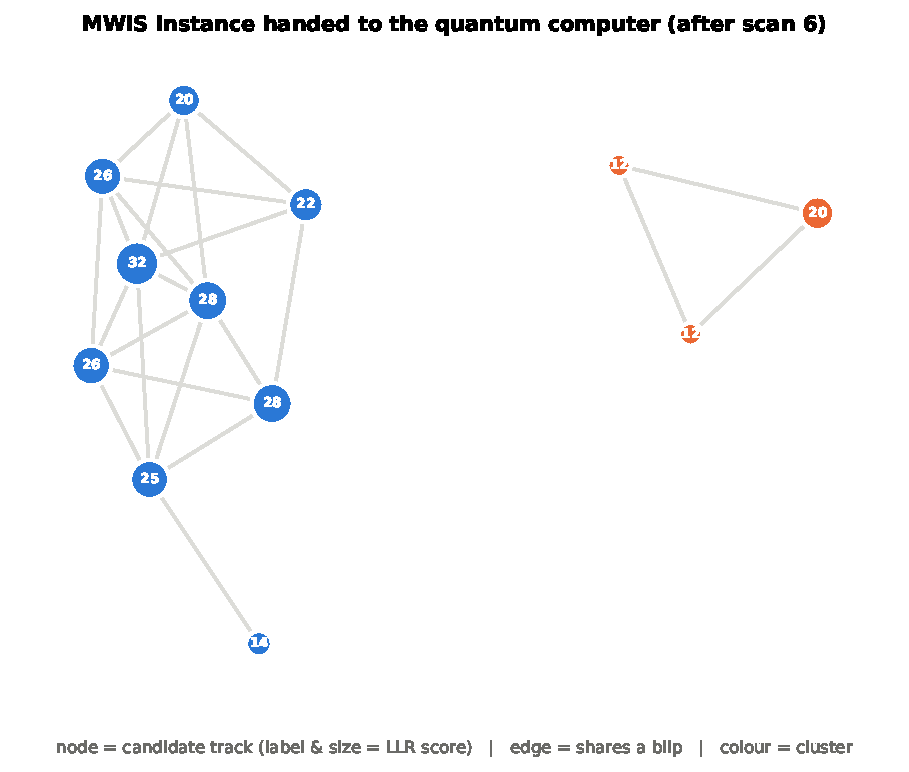
\includegraphics[width=\linewidth]{mwis_graph.pdf}
  \caption{An MWIS instance produced by the tracker. Vertices are candidate
  tracks (label and size give the LLR score), edges mark tracks sharing a
  detection, colour marks the cluster.}
  \label{fig:graph}
\end{figure}

\paragraph{Classical pruning is what makes it fit.} The largest cluster over a
whole scenario was $9$ vertices, far inside the $256$-atom device. Gating,
confirmation, track merging and $N$-scan pruning --- not the quantum step --- are
what keep the problem small. Removing track merging alone inflates clusters into
near-cliques that no planar atom register can represent.

\section{The geometric embedding}

This is the hard part. On the hardware one does not choose the edges: physics
decides them from distance, so the graph solved is always a \emph{unit-disk
graph}. An arbitrary MHT graph is not. We require
\begin{equation}
  \|p_i - p_j\| < R_b \ \text{(edge)}, \qquad
  \|p_i - p_j\| > R_b \ \text{(non-edge)},
\end{equation}
and solve this by penalty minimisation with random restarts, working in units of
$R_b$ and choosing the physical scale afterwards.

That last point matters. The layout fixes only distance \emph{ratios}; choosing
$R_b$ fixes everything else through Eq.~\eqref{eq:rb}. A larger $R_b$ gives the
atoms more room but costs Rabi frequency as $R_b^{-6}$, and too small an $\Omega$
never leaves the ground state within the device's $6\,\mu$s sequence limit. So
$\Omega$ is \emph{derived}, not chosen: we take the smallest $R_b$ respecting the
$5\,\mu$m tweezer spacing, then clamp it.

\begin{figure}[H]
  \centering
  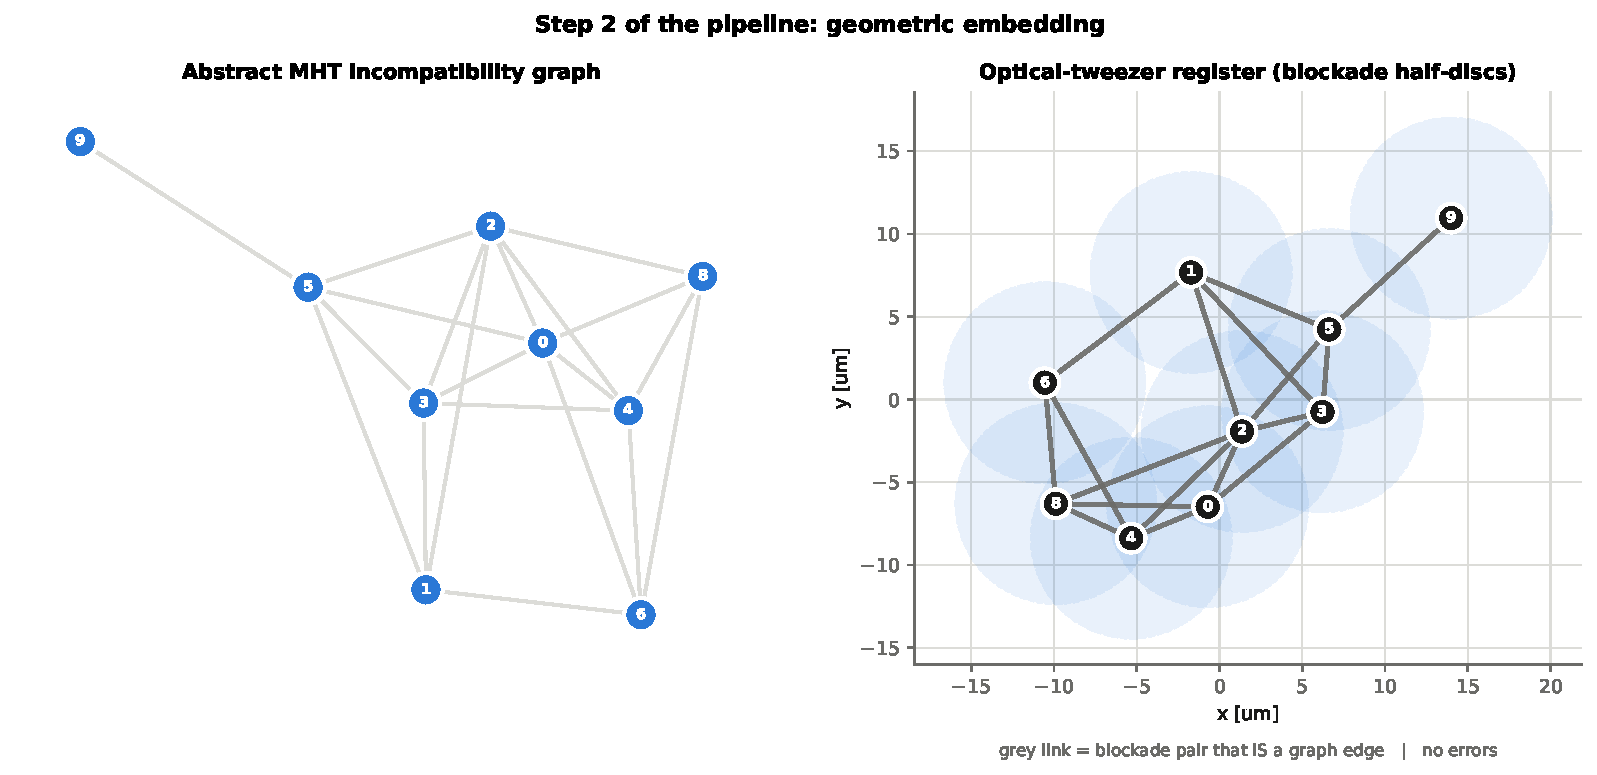
\includegraphics[width=\linewidth]{embedding.pdf}
  \caption{Abstract conflict graph (left) and the optical-tweezer register that
  realises it (right); shaded discs indicate the blockade range.}
  \label{fig:embed}
\end{figure}

\paragraph{Cliques are the obstruction.} A $k$-clique requires $k$ atoms pairwise
within $R_b$ yet pairwise at least $d_{\min}=5\,\mu$m apart. The feasible size
depends only on $\rho = R_b/d_{\min} \approx 2.4$. A regular hexagon plus its
centre gives seven points with ratio exactly $2$, so at least seven fit; the true
limit is around nine. Because branches of one family are mutually exclusive, each
family contributes a clique --- which is why capping branches per family is not a
tuning choice but a hardware constraint.

Figure~\ref{fig:embeddability} shows how quickly perfect embeddings disappear.

\begin{figure}[H]
  \centering
  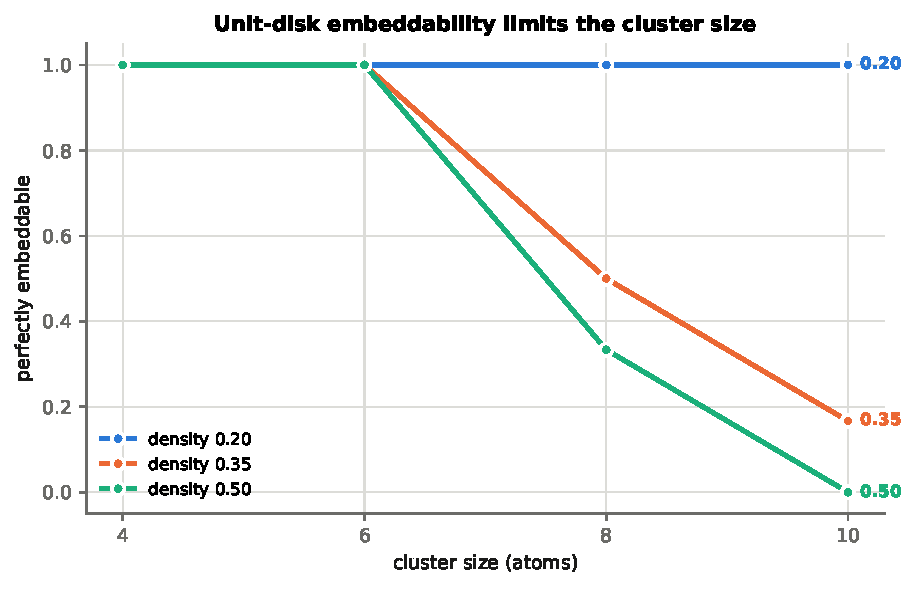
\includegraphics[width=\linewidth]{embeddability.pdf}
  \caption{Fraction of random graphs admitting a perfect unit-disk embedding.
  The binding limit is cluster size and density, not the $256$-atom capacity.}
  \label{fig:embeddability}
\end{figure}

\section{Validation}

We reproduce the worked example of~\cite{papa2009} (their Table 1 and Figure 5):
six tracks with published incompatibility lists and scores, of which five have
positive score. The published optimum is tracks $\{3,6\}$ with weight $19.2$. Our
classical solver and the atom array both return exactly this, the array sampling
it in $93$--$95\%$ of shots with a defect-free embedding. This is the only
external ground truth in the project.

In closed-loop tracking on synthetic radar data (five converging targets, $P_D =
0.9$, Poisson clutter), the array solved $21$ MWIS instances and matched the exact
classical optimum on all $21$, tracking all objects with $100\%$ association
accuracy.

\section{Testing the proposed advantage}

The optimisation works, but at these sizes a classical solver finds the optimum
instantly. The interesting claim concerns Eq.~\eqref{eq:probs}: the array should
supply a \emph{distribution} over hypotheses at fixed cost, whereas classical
enumeration cost grows with how many hypotheses exist (up to $3^{n/3}$).

We tested this on real data: the \texttt{PhC-C2DL-PSC} sequence from the Cell
Tracking Challenge~\cite{ctc}, $300$ frames of phase-contrast microscopy in which
pancreatic stem cells proliferate from $74$ to $661$. Detections come from the
raw images (background subtraction and connected components; recall $\approx
0.5$, precision $\approx 0.85$); the ground truth grades the detector only. From
these we built six MWIS instances of $9$--$12$ tracks.

\paragraph{Metric.} We measure the \emph{posterior mass} discovered per sample.
Counting distinct hypotheses would treat a $0.1\%$-probability explanation as
equal to one carrying $90\%$; Eq.~\eqref{eq:probs} does not. A ``sample'' is one
prepare--evolve--measure cycle for the array, one annealing run for simulated
annealing, one construction for randomised greedy. All three receive identical
post-processing.

\begin{table}[H]
  \centering
  \small
  \caption{Samples needed to capture $90\%$ of the posterior mass, averaged over
  six instances from real microscopy data.}
  \label{tab:route1}
  \begin{tabular}{lcc}
    \toprule
    Sampler & Samples & Precision \\
    \midrule
    Simulated annealing        & $\mathbf{23.6}$ & $98.0\%$ \\
    Neutral atoms (repaired)   & $27.5$          & $\mathbf{97.8\%}$ \\
    Randomised greedy          & $35.3$          & $91.0\%$ \\
    Neutral atoms (no repair)  & $32.2$          & $64.2\%$ \\
    \bottomrule
  \end{tabular}
\end{table}

\begin{figure}[H]
  \centering
  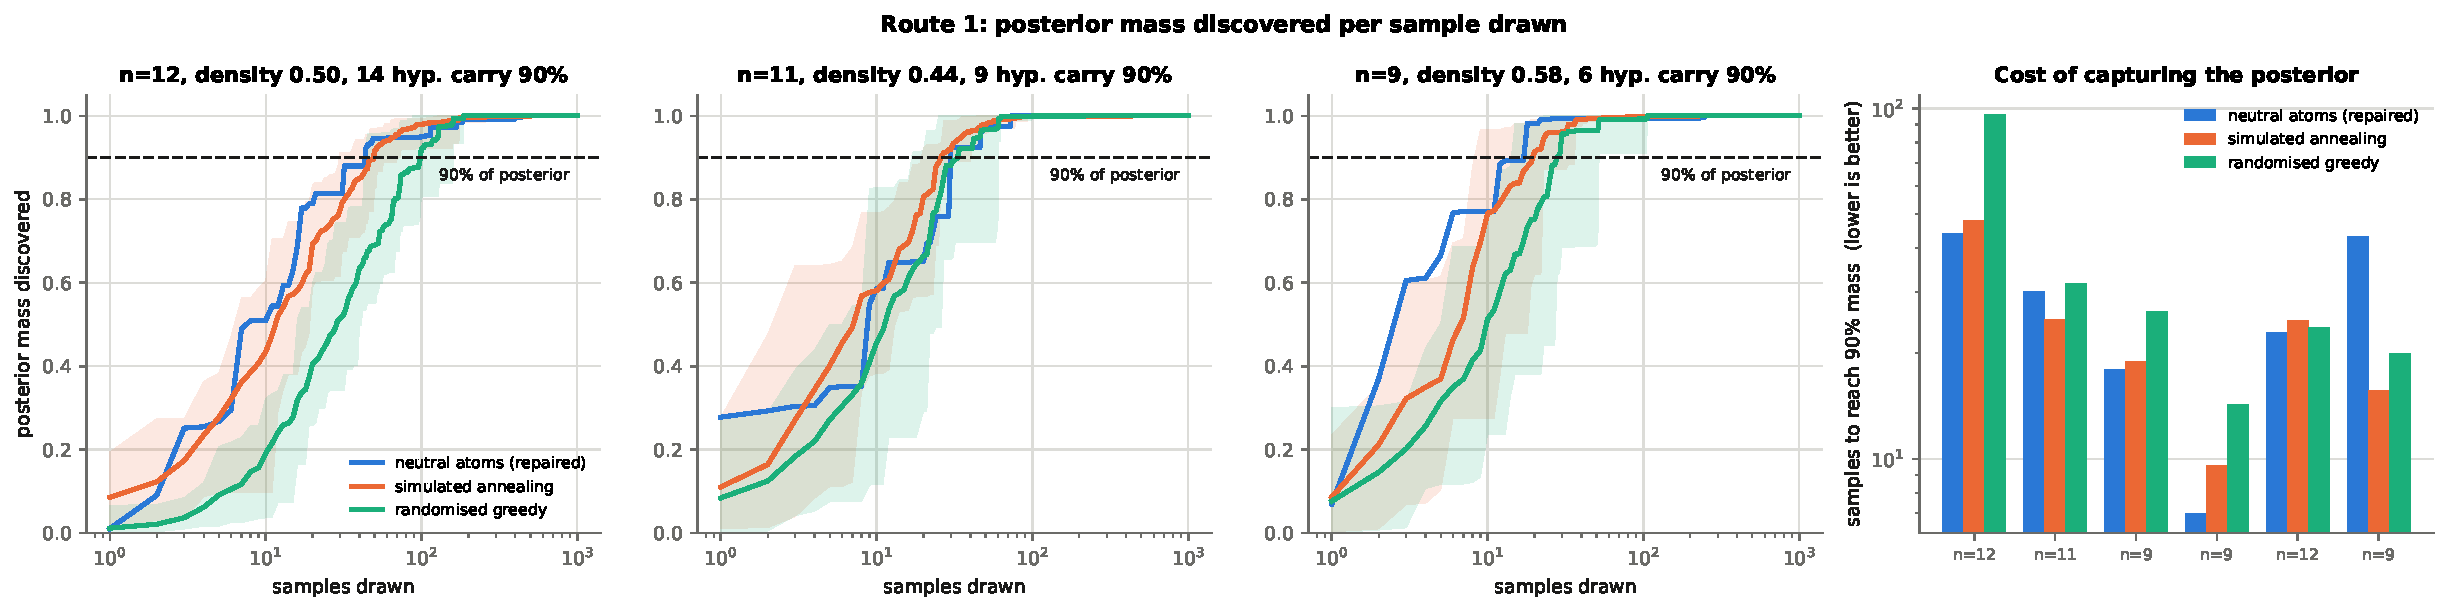
\includegraphics[width=\linewidth]{route1_curves.pdf}
  \caption{Posterior mass discovered against samples drawn.}
  \label{fig:route1}
\end{figure}

\paragraph{Result.} The claim is not supported. The array needed more samples
than simulated annealing on average, though the margin is small and the reading
should be ``indistinguishable at this sample size'' rather than a clear loss: the
array won on four of six instances individually, beat randomised greedy
comfortably, and annealing's lead vanishes when its budget is cut to two sweeps
per sample. Six instances cannot settle the question either way.

\section{Why, and what it implies}

\paragraph{Embeddability dominates.} The real conflict graphs had mean density
$0.66$, and $34\%$ of raw measurements violated an edge. The blockade --- the one
mechanism meant to enforce constraints for free --- was not enforcing them,
because the layout could not realise every edge. Classical repair then does that
work, and a repaired measurement is no longer a physical sample. This is exactly
what Fig.~\ref{fig:embeddability} predicts.

\paragraph{Concentration fights coverage.} Capturing $90\%$ of the posterior
needs about seven distinct hypotheses, but an adiabatic sweep is designed to
return one. Figure~\ref{fig:sweep} shows the trade: sweep duration moves
$P(\text{optimum})$ from $8\%$ to $99\%$ while diversity moves the other way. The
same register is an optimiser or a hypothesis generator depending only on how
fast it is driven --- a knob with no classical analogue, but not enough to close
the gap here.

\begin{figure}[H]
  \centering
  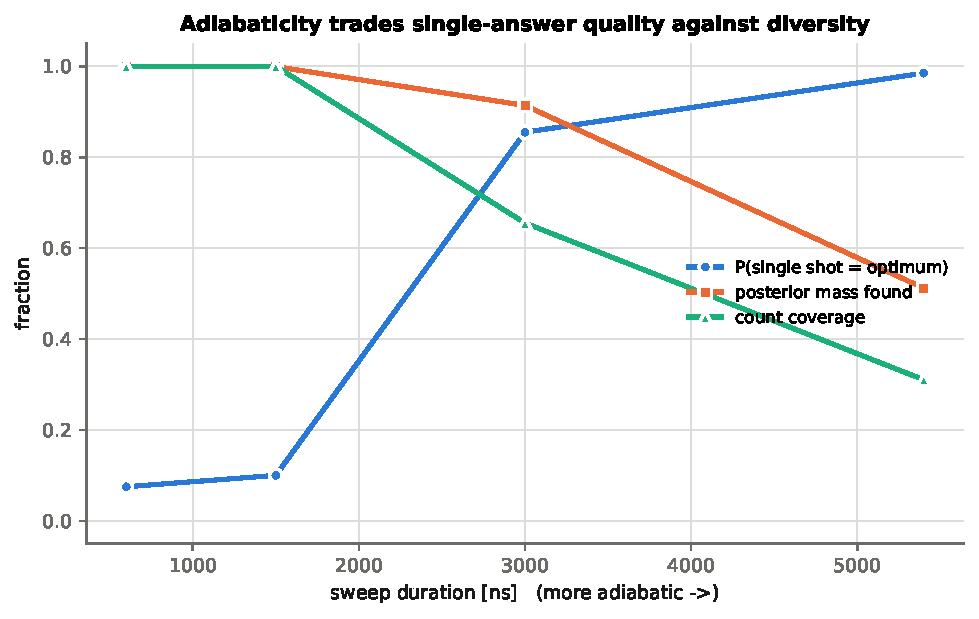
\includegraphics[width=\linewidth]{route1_sweep.pdf}
  \caption{Adiabaticity trades single-shot quality against diversity.}
  \label{fig:sweep}
\end{figure}

\paragraph{$\lambda$ is not a free parameter.} The QUBO penalty is $C_6/r_{ij}^6$,
fixed by atom placement. What one chooses is $\delta_{\max}/\Omega$, and it is
bounded on both sides: too small and the detunings cannot express weight
differences; too large and a blockaded pair profits from being excited together.
The measured usable window was $2 \lesssim \delta_{\max}/\Omega \lesssim 5.6$,
the upper bound being $r_{\text{edge}}^{-6}$.

\paragraph{Weight encoding is quantised.} The DMM cannot resolve arbitrarily
small local detunings, so score differences below about $2.6$ LLR are invisible
to the hardware.

\section{Conclusions}

The physics mapping is sound and the implementation reproduces published results
exactly. What does not follow is an advantage. The limiting factor is not qubit
count --- we never needed more than $12$ of $256$ atoms --- but geometry: MHT
conflict graphs are unions of cliques joined sparsely, and cliques are the worst
case for planar unit-disk embedding.

The useful consequence is that formulating the association problem so that the
graph is \emph{natively} unit-disk is a precondition, not a refinement. A
promising and untested direction is to place atoms according to proximity in
track state space, since tracks sharing a detection tend to be close there.

Open questions we did not resolve: the bias introduced by repairing measurements;
unresolved targets, where two objects merging into one detection should be
permitted to share it; and hardware noise, which attacks the weight encoding
directly because the weights \emph{are} detunings.

\begin{thebibliography}{9}\small
\bibitem{papa2009}
D.~J.~Papageorgiou and M.~R.~Salpukas,
\emph{The Maximum Weight Independent Set Problem for Data Association in Multiple
Hypothesis Tracking}, in Optimization and Cooperative Control Strategies,
Springer, 2009, pp.~235--255.

\bibitem{ctc}
V.~Ulman \emph{et al.},
\emph{An objective comparison of cell-tracking algorithms},
Nature Methods \textbf{14}, 1141--1152 (2017).
Dataset \texttt{PhC-C2DL-PSC}, \url{http://celltrackingchallenge.net}.

\bibitem{pulser}
H.~Silv\'erio \emph{et al.},
\emph{Pulser: An open-source package for the design of pulse sequences in
programmable neutral-atom arrays}, Quantum \textbf{6}, 629 (2022).

\bibitem{ebadi}
S.~Ebadi \emph{et al.},
\emph{Quantum optimization of maximum independent set using Rydberg atom arrays},
Science \textbf{376}, 1209--1215 (2022).
\end{thebibliography}

\end{document}
